\documentclass[11pt]{article}
\usepackage{amsmath,amsfonts,amssymb}
\usepackage{hyperref}
\hypersetup{
	colorlinks=true,
	linkcolor=blue,
	urlcolor=cyan
	}
\usepackage[margin=1in]{geometry}
\usepackage{graphicx}

\setlength{\parindent}{0pc}
\setlength{\parskip}{10pt}

\title{STAT157 HW 3}
\date{Jan 31, 2022}

\begin{document}

\maketitle

\hfill \textbf{Due Monday, February 7 at 11:59pm}

\section*{Deliberate Practice: Zeroth and First Order Forecasting}

\emph{Expected completion time: 60 minutes}

For each of the following time series, estimate the value of the next few points without looking things up, then look at your answers and report your relative errors. You will be graded on your thinking process, not your accuracy.

\begin{enumerate}
	\item Energy usage until January 30, 2022
	
	
	\begin{itemize}
		\item To find the graph, go to \href{https://www.eia.gov/electricity/gridmonitor/expanded-view/electric_overview/US48/US48/ElectricityOverview-2/edit}{this link}, in ``Chart options'' and ``Date Range Type'' select ``Custom'', and in ``Date Range'' enter ``01/01/2022 - 01/31/2022''.
		\item Predict energy usage for every day of the week from Jan 31 to Feb 7 at 11am SF time.
	\end{itemize}
	
	\item Number of full-time Facebook employees until 2016
	
	\begin{center}	
		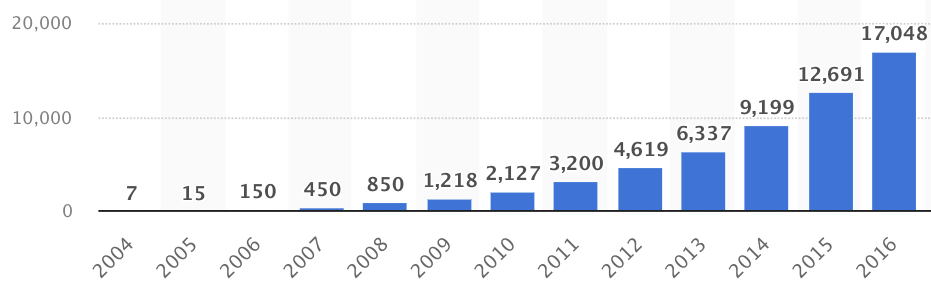
\includegraphics[width = 375px]{2.png}
	\end{center}

	\begin{itemize}
		\item Predict the number of full-time employees in 2017, 2018, 2019, and 2020.
	\end{itemize}
	
	\item Total adult correctional population until 2010

	\begin{center}	
		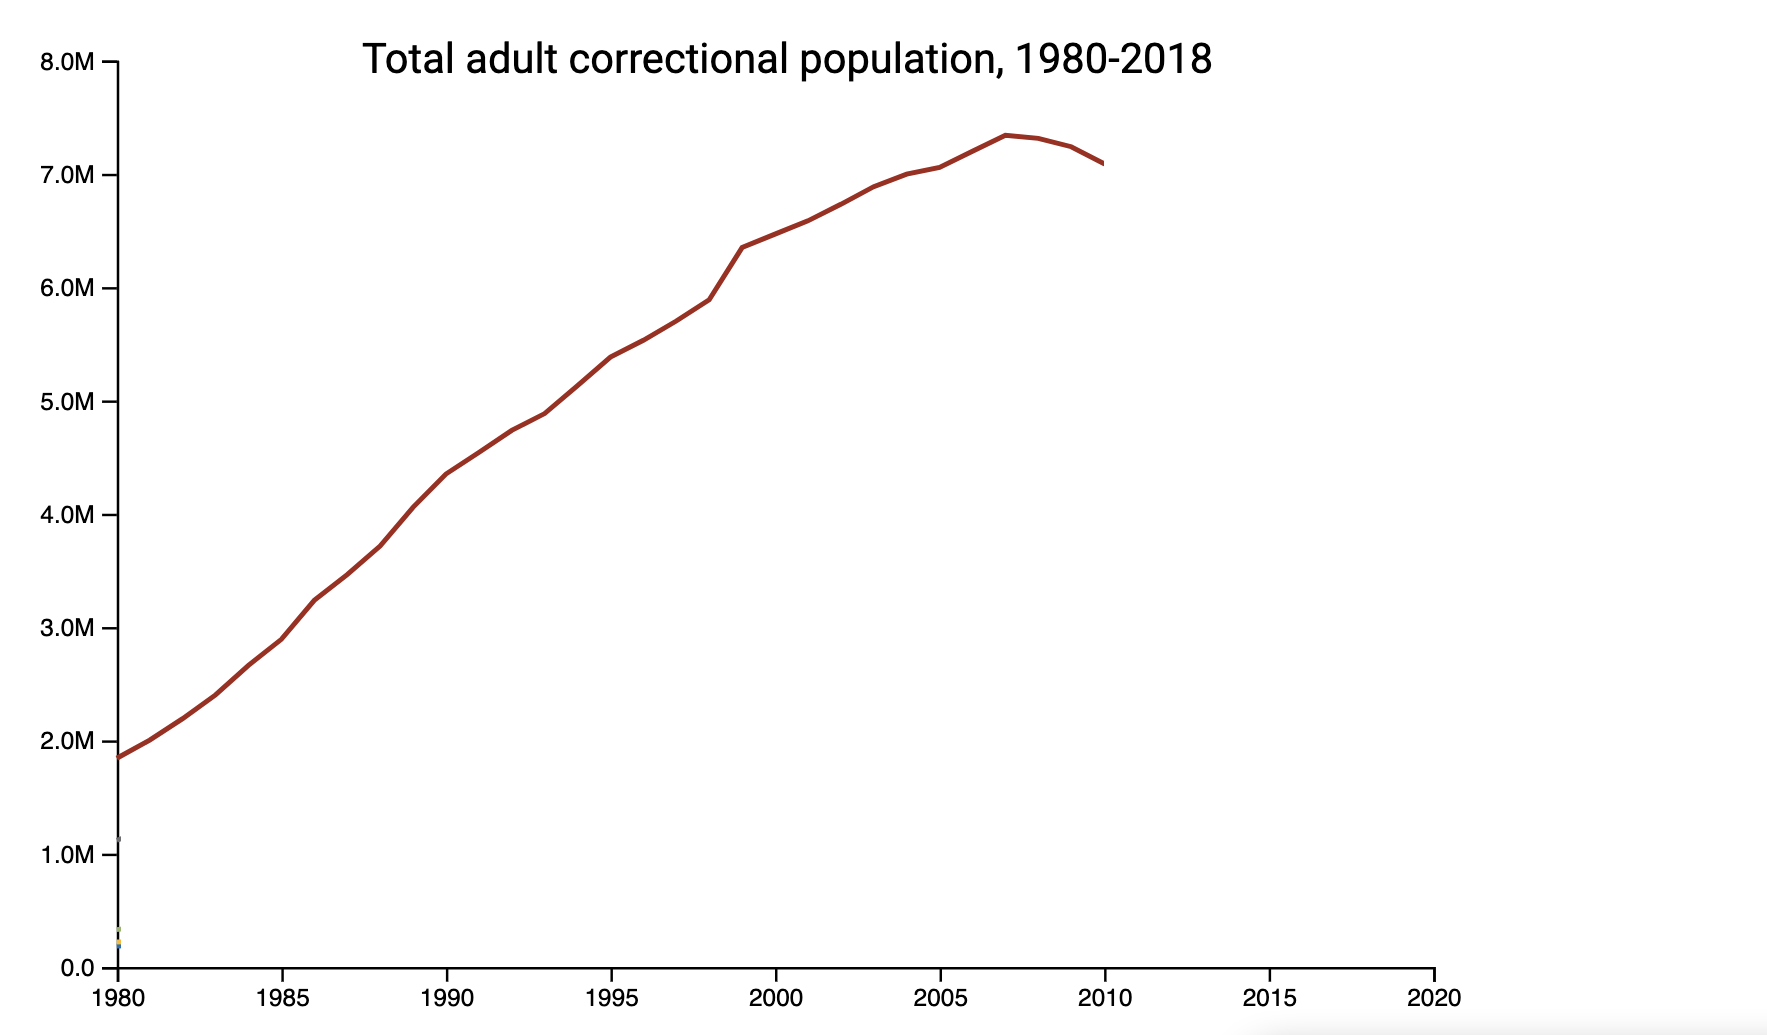
\includegraphics[width = 375px]{3.png}
	\end{center}


	\begin{itemize}
		\item Predict the adult correctional population in 2012, 2014, 2016, and 2018.
	\end{itemize}
	
	\item World GDP until 1950
	\begin{itemize}
		\item \href{https://ourworldindata.org/grapher/world-gdp-over-the-last-two-millennia?time=1..1950}{Link} to the graph.
		\item Predict World GDP in 1955, 1960, 1970, and 1990.
	\end{itemize}
	
	\item TSA passenger throughput numbers until Jan 30, 2022

	\begin{center}	
		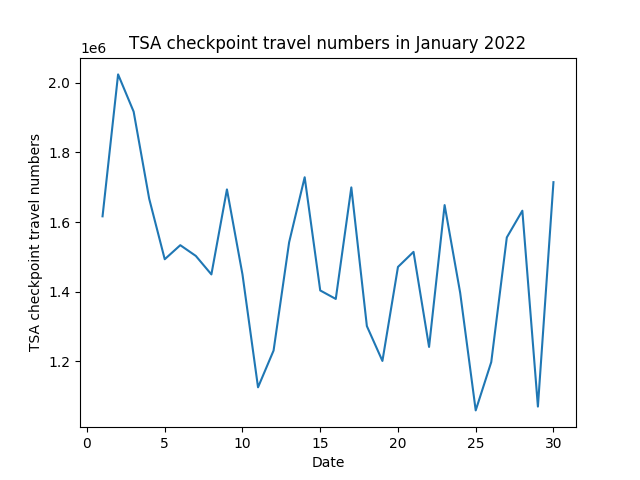
\includegraphics[width = 375px]{tsa_checkpoint.png}
	\end{center}

	\begin{itemize}
		\item This graph uses the January 2022 numbers from \href{https://www.tsa.gov/coronavirus/passenger-throughput}{here}.
		\item Predict the passenger throughput number for Feb 7.
	\end{itemize}
	
	\item Per capita C02 emissions in US until 2010
	\begin{itemize}
		\item \href{https://ourworldindata.org/grapher/co-emissions-per-capita?tab=chart&time=1750..2010&country=~USA}{Link} to the graph.
		\item Predict the US per capita C02 emissions in 2015, 2020, 2025, and 2030.
	\end{itemize}
	
	\item Military expenditure as a percent of GDP until 2012
	\begin{itemize}
		\item \href{https://ourworldindata.org/grapher/military-expenditure-share-gdp-sipri?time=earliest..2012&country=~USA}{Link} to the graph.
		\item Predict military expenditure as a percent of GDP in 2015, 2018, and 2019.
	\end{itemize}

	\item Worldwide total fertility rate until 1978
	\begin{itemize}
		\item \href{https://ourworldindata.org/grapher/children-per-woman-UN?tab=chart&time=1950..1978}{Link} to the graph.
		\item Predict the worldwide total fertility rate in 1983, 1988, 1993, 1998, and 2003.
	\end{itemize}
	
	\item US Child mortality rate until 1955
	\begin{itemize}
		\item \href{https://ourworldindata.org/grapher/child-mortality?time=earliest..1955&country=~USA}{Link} to the graph.
		\item Predict the child mortality rate in 1960, 1970, 1980, 1990, and 2010.
	\end{itemize}
\end{enumerate}

On Gradescope, for each of the \textbf{9 questions}, submit your estimates, reasoning and relative errors. Please also submit the time it took to complete this exercise.

\section*{Deliberate Practice: Estimation and Calibration}

\emph{Expected completion time: 45 minutes}

For each of the following questions, estimate an inclusive $80\%$ confidence interval for the answer without looking things up. For each quantity, we provided one link with a reasonable-seeming answer. We recommend spending around 5-10 minutes on each estimation question. You will be graded on your thinking process, not your accuracy.

\begin{enumerate}
	\item How many employment-based Green Card applications did US Citizenship and Immigration Services process in 2021? Note that the question is about the number of applications \emph{processed}, not \emph{approved}. \href{https://www.uscis.gov/newsroom/news-releases/uscis-announces-fy-2021-accomplishments}{Link to Answer}
	\item How many acres of US land were burnt by wildfires in 2020? \href{https://sgp.fas.org/crs/misc/IF10244.pdf}{Link to Answer}
	\item How many records have the Beatles sold, in terms of worldwide certified (not claimed) sales, as reported by Wikipedia? Records include singles and full-length albums. \href{https://en.wikipedia.org/wiki/List_of_best-selling_music_artists#250_million_or_more_records}{Link to Answer}
	\item What is TSMC's projected \href{https://en.wikipedia.org/wiki/Capital\_expenditure}{capex} for 2022 in dollars? \href{https://www.reuters.com/technology/tsmc-q4-profit-rises-164-record-beats-market-forecasts-2022-01-13/}{Link to Answer}
	\item How many metric tons of crude oil were produced worldwide in 2020? \href{https://www.statista.com/statistics/265229/global-oil-production-in-million-metric-tons/#:~:text=In$\%$202020$\%$2C$\%$20global$\%$20crude$\%$20oil,about$\%$204.2$\%$20billion$\%$20metric$\%$20tons}{Link to Answer}
\end{enumerate}

On Gradescope, for each of the \textbf{5 questions}, submit your estimate and an explanation of your reasoning. Please also submit the time it took to complete this exercise.

\section*{Deliberate Practice: Reference Classes}

\emph{Expected completion time: 60 minutes}

For the following questions, describe 3 reference classes you would use to answer it, and what estimates they lead to. To do this, you can look up information about the reference classes, but not the answer itself. 

Once you have come up with the reference classes, look up the answer, and discuss which reference classes worked well, and which worked poorly. We recommend spending around 15 minutes on each question.

\begin{enumerate}
	\item How much did the movie \emph{Harry Potter and the Deathly Hallows - Part 2} gross worldwide? \href{https://en.wikipedia.org/wiki/Harry_Potter_and_the_Deathly_Hallows_%E2%80%93_Part_2#Box_office}{Link to Answer}
	\item A diplomatic boycott of a competition is when a country does not send high-ranking officials to attend the competition as official representatives, but still sends athletes. How many countries issued a diplomatic boycott of the 2022 Winter Olympics in China by January 31? \href{https://en.wikipedia.org/wiki/2022_Winter_Olympics#Diplomatic_boycotts}{Link to Answer}
	\item What was Delta Air Lines' \href{https://www.investopedia.com/terms/o/operating-revenue.asp}{operating revenue} in 2020? \href{https://ir.delta.com/news/news-details/2021/Delta-Air-Lines-Announces-December-Quarter-and-Full-Year-2020-Financial-Results/default.aspx}{Link to Answer}
	\item How many years were there between the beginning and end of the construction of the \href{https://en.wikipedia.org/wiki/Sydney_Opera_House#/media/File:Sydney_Australia._(21339175489).jpg}{Sydney Opera House}? \href{https://en.wikipedia.org/wiki/Sydney_Opera_House}{Link to Answer}
	
\end{enumerate}

On Gradescope, for each of the \textbf{4 questions}, submit your reference classes and reasoning. Please also submit the time it took to complete this exercise.

\section*{Predictions}

\emph{Expected completion time: 60 minutes}

Register the following predictions. You can submit them by going to \url{https://forms.gle/yJsQoMaWYXjzfwRt5} and following the form's instructions. For these predictions, (and all predictions about the future throughout this class), we encourage you to use external sources -- by googling things, reading news articles, talking to friends who follow politics or music stats, etc.

\begin{enumerate}
	\item[0.] Pick the same website, application, or software you chose last week, and predict how much time you will spend on it between 12:00am Tuesday February 8th and 11:59pm Sunday February 13th., as measured by your time-tracking app.

	\item[1.] How many medals will the US have in the Winter Olympics by Sunday Feb 13 2022 at 11:59pm SF time?
	
	\item[2.] What will the price of Ethereum be on Sunday Feb 13 2022, as reported by \href{https://www.coinbase.com/price/ethereum}{Coinbase} at 11:59pm?
 
	\item[3.] Will California announce an extension of the current indoors mask mandate to beyond Feb 15 between Monday Feb 7 at 11:59pm and Sunday Feb 13 at 11:59pm?
	
	\item[4.] Which player will have the most points per game of the 2021-2022 NBA season by Sunday Feb 13? This resolves as whoever tops \href{https://www.nba.com/stats/players/traditional/?sort=PTS&dir=-1&Season=2021-22&SeasonType=Regular%20Season}{this leaderboard} on February 13 at 11:59pm.
	
	
\end{enumerate}

For each question, submit a mean and inclusive 80\% confidence interval (or a probabilities for questions 3 and 4), as well as an explanation of your reasoning (~1-2 paragraphs). \textbf{Please include a copy of your google form responses with your Gradescope submission.} On Gradescope, please also submit the time it took to complete this exercise.


\end{document}